\chapter{Dataset Reconstruction and Analysis}
\label{cha:3}

This chapter discusses the chosen dataset for this study, the BAT dataset. It includes details on the dataset's analysis, cleaning, and reconstruction through crawling article contents.

\section{The BAT dataset} \label{bat-characteristics}

The BAT dataset \cite{spinde-2023-bat} contains 6,345 rows of manually labelled news articles published by 255 English-speaking news outlets (US-based), originally scraped from Ad Fontes Media's website. Articles in the dataset encompassed a wide range of topics such as COVID-19, politics, and lifestyle. This dataset was chosen for this project primarily because of its political bias and reliability scores, which provide a clear and useful label for classifying media bias at the article level.

The political bias score measures the extent of political influence, ranging from -42 (most extreme left) to +42 (most extreme right), reflecting the article's truthfulness, with values ranging from 0 (least reliable, containing inaccurate or fabricated information) to 64 (most reliable, original fact reporting) \cite{adfontes-bias-reliability}. The reliability score evaluates original fact reporting to analysis, opinion, propaganda, and inaccurate/fabricated information, with scores above 40 generally considered good and scores below 24 typically seen as problematic, scores between 24 and 40 suggest a variety of factors, including a strong presence of opinion and analysis or significant variability in reliability across different articles \cite{adfontes-bias-reliability}.

Ad Fontes rates articles using a politically balanced panel consisting of at least three analysts representing right-leaning, centrist, and left-leaning perspectives. The scores from each analyst are compared, and any discrepancies are discussed and adjusted if necessary, before averaging to obtain the final rating \cite{adfontes-methodology}. No further information can be found regarding their specific values and range of these rating, it can be safely assumed that this is an inherent part of their algorithms and methodology.

The reliability score is selected as the label in this project because it measures truthfulness and original fact reporting. Articles with high reliability scores typically do not exhibit any textual-level biases, such as phrasing bias, spin bias, or statement bias, as described in Chapter \ref{cha:2}.

\begin{figure}[htbp]
    \centering
    \begin{minipage}{1\linewidth}
        \begin{center}
            \small{\textbf{Trenton police officer takes own life in Plainsboro parking lot, officials say}}
        \end{center}
        \scriptsize{
            A veteran Trenton police officer took his own life in a parking lot Wednesday, officials said. Sgt. Daniel Pagnotta, a 21-year-veteran of the department, died this morning in Plainsboro, according to a city spokesman.“Beloved by everyone in the Trenton Police Department, he was devoted to Trenton and police work,” Mayor Reed Gusciora said in a statement. The statement described Pagnotta as a devoted husband and father of two who loved soccer and making people laugh. His father, also named Dan, is a retired Trenton police officer.“Dan was proud to continue a legacy of law enforcement in his family,” Gusciora said. “Dan and his family are on our minds and in our hearts. He will be dearly missed.”}
    \end{minipage}
    \caption{Example of a non-biased article, reliability score: 57.67}
    \label{fig:example-nonbiased-article-1}
\end{figure}

\begin{figure}[htbp]
    \centering
    \begin{minipage}{1\linewidth}
        \begin{center}
            \small{\textbf{Army Rejects Mike Flynn’s Call For Trump To Declare Martial Law And Overturn The Election}}
        \end{center}
        \scriptsize{
            After Mike Flynn called for Trump to declare martial law and overturn the election, Army leadership flatly rejected the idea. The Army response to Flynn’s fascist idea was to reject it: The military has made it very clear that they will not be participating in any last-ditch attempts by Trump to destroy democracy to stay in power. Flynn’s idea that Trump should overturn the election shows that Trump and his associates have always been anti-democratic. They don’t respect democracy or view it as their role to uphold and promote democratic institutions in the United States. There is not going to be any declaration of martial law. Trump isn’t going to overturn the election. Trump is not going to get help from the military to stay in power. The soon to be former president was the face of the fascist threat, but he has converted the Republican Party into an anti-democratic movement for autocracy. Donald Trump lost, but the authoritarian impulse behind Trumpism still must be defeated for democracy in the United States to be saved.}
    \end{minipage}
    \caption{Example of a non-biased article, reliability score: 30.0}
    \label{fig:example-mixed-biased-article-1}
\end{figure}

\begin{figure}[htbp]
    \centering
    \begin{minipage}{1\linewidth}
        \begin{center}
            \small{\textbf{Is the FBI corrupt beyond repair?}}
        \end{center}
        \scriptsize{
            Last week, the most recent slap in the face to the American people came in the form of a corrupt FBI lawyer getting a fine less than seatbelt ticket for falsifying documents to violate the civil rights of American citizens. Unfortunately, this is the latest in a laundry list of issues with the FBI. The most glaring problem with the FBI is its actions during the Russia Collusion hoax. The FBI allowed itself to become the enforcement arm of the Democratic Party. There is a slim chance the law enforcement agency did not know it was being used initially, but it had to know it was being used shortly after the 2016 election...
        }
    \end{minipage}
    \caption{Example of a biased article, reliability score: 6.67}
    \label{fig:example-biased-article-1}
\end{figure}

An example of a highly-rated article can be seen in Figure \ref{fig:example-nonbiased-article-1}. The article reports only factual information regarding the event and includes statements from people related to the incident. It contains no journalist opinions or political innuendos. In contrast, an example of a low-rated article can be seen in Figure \ref{fig:example-biased-article-1}. The article refers to the event as "the most recent slap in the face," which exemplifies phrasing bias. Additionally, the author's negative view of the FBI is evident, indicating a statement bias. Lastly, Figure \ref{fig:example-mixed-biased-article-1} shows an article that is rated in the middle quartile with a reliability score of 30.0. The article uses strong language, such as "fascist," and makes a broad assumption, claiming that Trump is anti-democratic. While the points raised in the article may have elements of truth, the way they are presented lacks balance and neutrality.

\section{Reconstruction}

The original BAT dataset contains the titles and URLs of articles but missing the full content. Therefore, it is necessary to crawl the websites to retrieve the complete article content. To address this, a Python script was developed to iteratively visit each URL in the dataset and extract the textual content. The initial round yielded 5,270 articles from the original 6,345 articles, with substantial data loss attributed to unavailable websites, missing articles, and broken links. Additionally, some pages could not be crawled by the script due to structural differences and had to be manually copied and pasted.

Subsequently, a second round of data retrieval was conducted by re-examining 1,075 articles that were not successfully crawled in the initial round. Each of these cases was individually investigated: missing articles were sought through public archives, broken links were repaired, using proxies to bypass geographical restrictions. Articles that were successfully retrieved were added to the dataset, resulting in an additional 226 articles. Thus, the final dataset contains 5,497 articles.

The extracted text contains noise, which upon inspection is categorised into two different types: \textbf{word-level noise} and \textbf{phrase-level noise} as illustrated in Table \ref{table:conjoined_words} and Table \ref{table:noise_phrases}. Word-level noise includes typing errors and conjoined words, mostly attributed to word links or texts with unusual HTML format that are difficult to cleanly extract. Phrase-level noises are attributed to extraneous content such as author information, subscription prompts, and donation appeals within the article text.

\begin{table}[htbp]
    \centering
    \small
    \begin{tabular}{| c | c | c |}
        \hline
        Newsreported           & saidon        & admittedthat       \\
        \hline
        TheNational            & 2021According & theirwithholdingis \\
        \hline
        statementthat          & DakotaToni    & Democrattoldthe    \\
        \hline
        DemocratsThe           & whatreporter  & PresidentVladimir  \\
        \hline
        Bidensaid              & whohas        & theDemocrats       \\
        \hline
        includingthe           & saidRep       & toreopen           \\
        \hline
        2021Trump              & Americanswho  & duringhis          \\
        \hline
        thecoronaviruspandemic & toMissouri    & toReuters          \\
        \hline
        haspreviously          & Postcolumnist & 2ndAmendment       \\
        \hline
    \end{tabular}
    \caption{Example of word-level noise, over sixty-thousand occurrences are found within the dataset article contents}
    \label{table:conjoined_words}
\end{table}

\begin{table}[htbp]
    \centering
    \scriptsize
    \begin{tabular}{| l |}
        \hline
        By submitting your email, you agree to our Terms and Privacy...                                        \\
        \hline
        ByChris MurphyByNick BiltonByErin Vanderhoof                                                           \\
        \hline
        Get a brief on the top business stories of the week, plus CEO interviews...                            \\
        \hline
        Kevin Winter/Getty Images                                                                              \\
        \hline
        Subscribe to our free News Alerts newsletter. Want more of our free, weekly newsletters in your inbox? \\
        \hline
        Join the 3,900+ MTFP members who believe in the power of independent news...                           \\
        \hline
        We're hiring! Please take a look at the new openings in our newsroom...                                \\
        \hline
        BYPASS THE CENSORSSign up to get unfiltered news delivered straight to your inbox                      \\
        \hline
        RealClear PoliticsLiz Peek writes about business and government. Submit a letter...                    \\
        \hline
        Follow Stephen Robinson onTwitter. Want to just donate once?                                           \\
        \hline
        At Vox, we believe that clarity is power, and that power shouldn’t only be available to those...       \\
        \hline
    \end{tabular}
    \caption{Examples of phrase noises, mostly subscription and donation prompts, that were inadvertently crawled into the article content.}
    \label{table:noise_phrases}
\end{table}

To identify word-level and phrase-level noises, the entire content of every article in the dataset was combined and tokenised, then matched with an English word list \cite{dwyl-english-words}, generating an error list that includes words found in the articles but not present in the dictionary. Entries in this error list were manually inspected, prioritising commonly occurring items. Based on these findings, scripts were developed to address both word-level and phrase-level noise. This process was iteratively repeated to correct as many issues as possible. However, due to project time constraints, it was impractical to resolve all identified and potential noises, which would have required extensive time and manual effort.

A total of 5,761 word-level noises were corrected, and 625 phrase-level noises were identified and stripped from article contents. The total of word-level noises that exist within the dataset is predicted to be over sixty-thousands occurrences, based on the error list. Pseudocode of the scripts can be seen in Algorithm \ref{alg:phrase_level_noise_fix} and \ref{alg:word_level_noise_fix} (Appendix \ref{app:A}).


\begin{table}[htbp]
    \centering
    \footnotesize
    \begin{tabular}{| c | c | c | c | c |}
        \hline                            \textbf{Method} & \textbf{Class}     & \textbf{Precision} & \textbf{Recall} & \textbf{F1} \\\cline{1-5}

        \multirow{5}{*}{BERT FT, before noise cleaning}   & Problematic        & 0.43               & 0.37            & 0.40        \\
                                                          & Questionable       & 0.33               & 0.39            & 0.36        \\
                                                          & Generally Reliable & 0.39               & 0.53            & 0.45        \\
                                                          & Reliable           & 0.91               & 0.81            & 0.86        \\\cline{2-5}
                                                          & Overall            & 0.7379             & 0.6994          & 0.7147      \\
        \hline
        \multirow{5}{*}{BERT FT, after noise cleaning}    & Problematic        & 0.43               & 0.44            & 0.44        \\
                                                          & Questionable       & 0.29               & 0.39            & 0.33        \\
                                                          & Generally Reliable & 0.44               & 0.48            & 0.46        \\
                                                          & Reliable           & 0.90               & 0.83            & 0.86        \\\cline{2-5}
                                                          & Overall            & 0.7359             & 0.7065          & 0.7193      \\
        \hline
    \end{tabular}
    \caption{Performance before and after noise cleaning of BERT fine-tuning}
    \label{table:noise_performance_comparison}
\end{table}

To evaluate the effects of the noise-cleaning procedure, a simple BERT fine-tuning approach is performed on the dataset with and without noise. As shown in Table \ref{table:noise_performance_comparison}, the cleaned dataset results in a slight improvement in both recall and F1 scores, along with a minor reduction in precision. This outcome is expected, as only a portion of the noise in the dataset was addressed. Continuation in further noise cleaning is projected to yield more pronounced improvements in performance.


\section{Analysis}

\begin{figure}[htbp]
    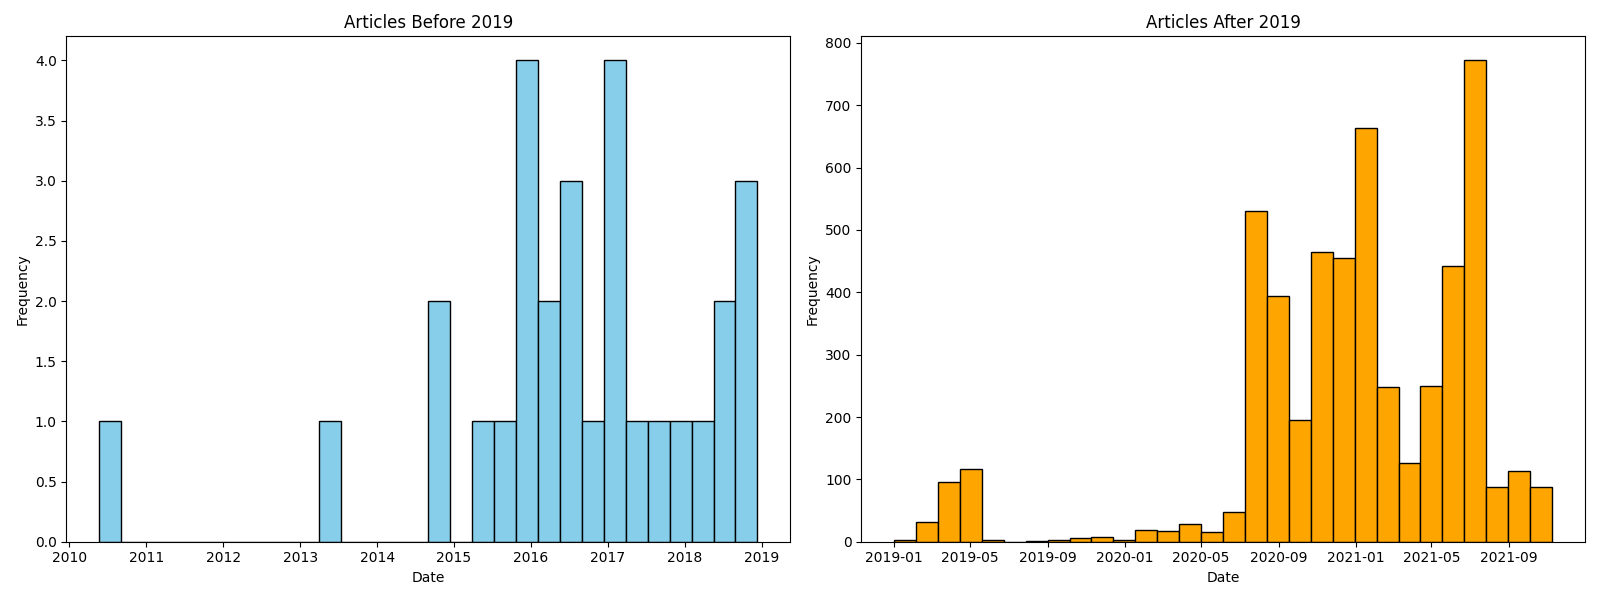
\includegraphics[width=\linewidth]{figures/dates_hist.png}
    \caption{Articles published date histogram.}
    \label{fig:dates_hist}
\end{figure}

Most articles in the BAT dataset were written and published within the last six years, with only thirty-one articles published before 2019 (Figure \ref{fig:dates_hist}). Looking at these articles individually, they generally cover similar topics to those published after 2019 and therefore should not exhibit consequential differences in behaviour and characteristics.

\begin{figure}[htbp]
    \centering
    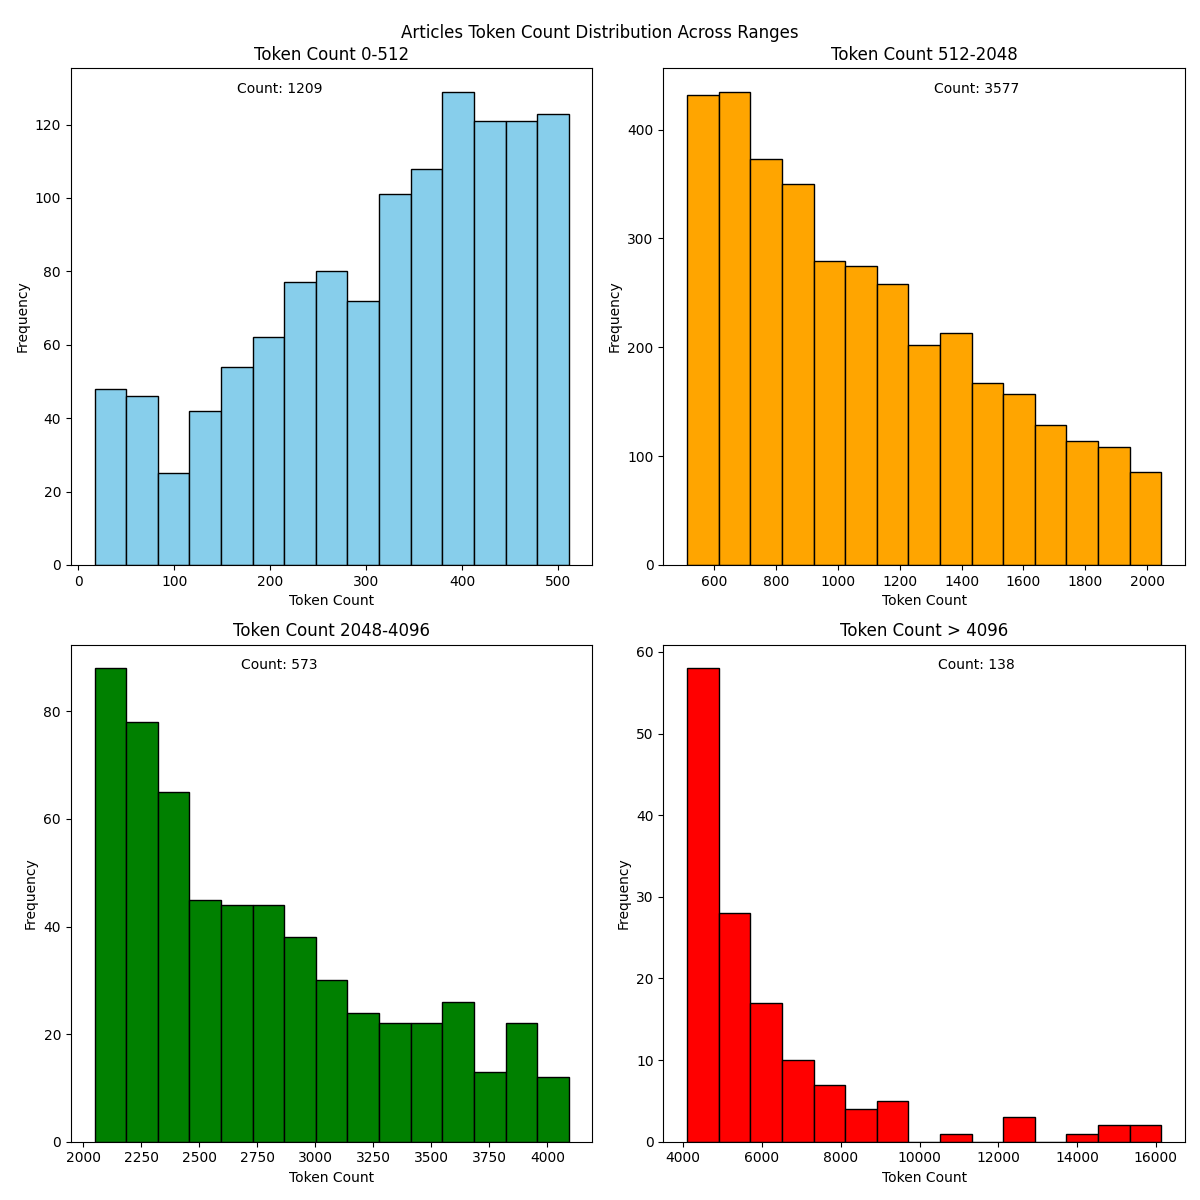
\includegraphics[width=0.9\linewidth]{figures/token_count_vx_split_hist.png}
    \caption{Articles tokens count distribution}
    \label{fig:token_hist_split}
\end{figure}

Analysis of articles token count can be seen in Figure \ref{fig:token_hist_split}. Note that sub-words are used as tokens in this analysis rather than whole words. The length of article content tokens ranges from 17 to 16,139, with an average length of 1,207.07 and a median value of 908 tokens. More than half of articles in the dataset have between 512 and 2,048 tokens. Only nine articles have more than 10,000 tokens, while 106 articles have fewer than 100 tokens. Furthermore, 1,209 articles contain 512 tokens or fewer, which is the maximum input length for BERT. Thus, when using BERT in its standard configuration, significant information loss is to be expected due to the token limit.

\begin{figure}[htbp]
    \centering
    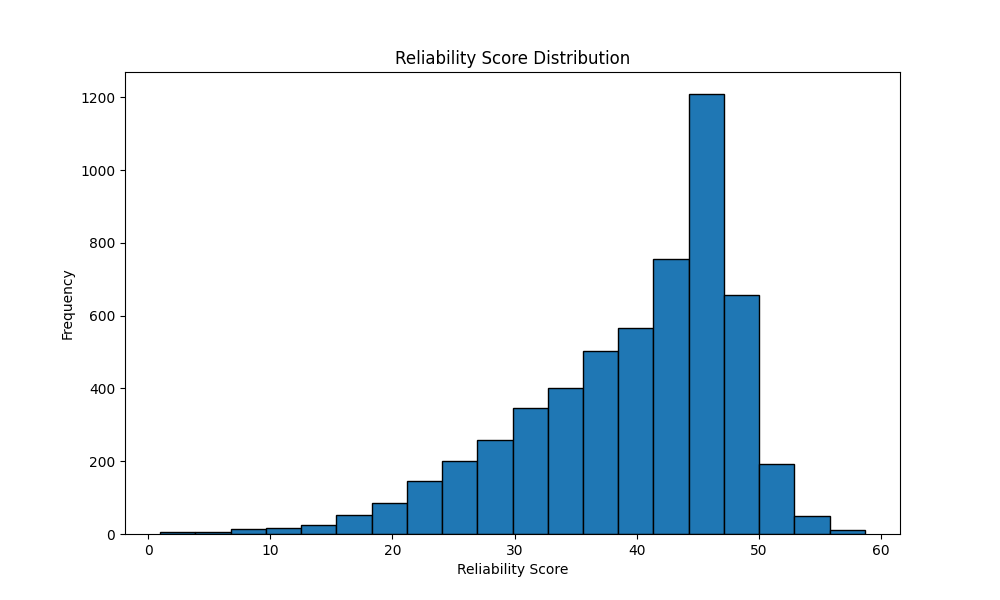
\includegraphics[width=0.9\linewidth]{figures/reliability_score_hist.png}
    \caption{Reliability score distribution}
    \label{fig:reliability_score_hist}
\end{figure}

The articles reliability scores range from 1.0 to 58.67, with the majority scoring between 40 and 50. No articles  exceed a score of 60, despite the highest possible score being 64. Thus, only several hundreds of articles are rated low. The full histogram of the reliability scores is shown in Figure \ref{fig:reliability_score_hist}.

\begin{figure}[htbp]
    \centering
    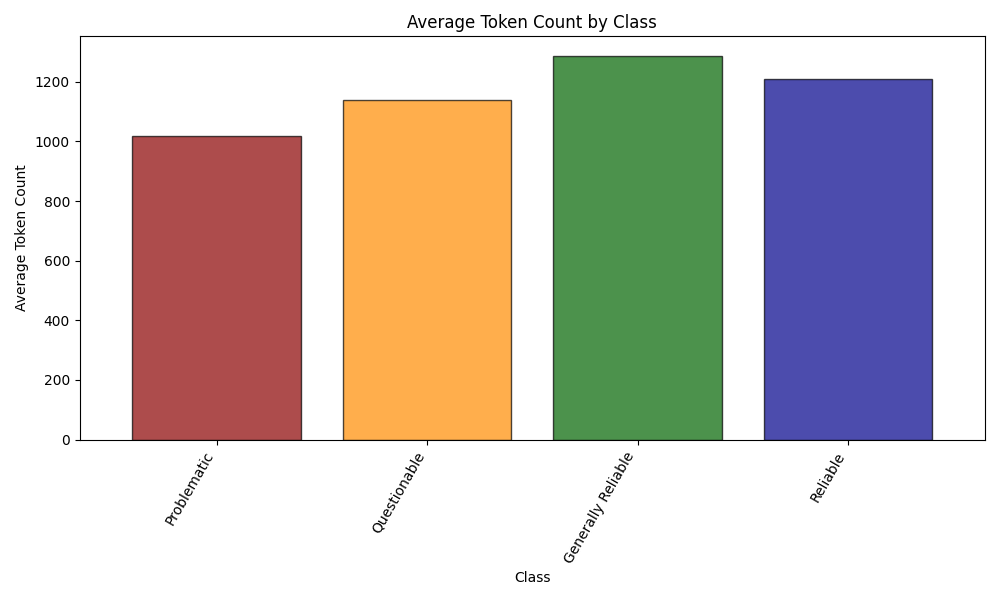
\includegraphics[width=0.7\linewidth]{figures/token_count_vx_per_class_hist.png}
    \caption{Average token count per class.}
    \label{fig:avg_token_per_class}
\end{figure}
\begin{figure}[htbp]
    \centering
    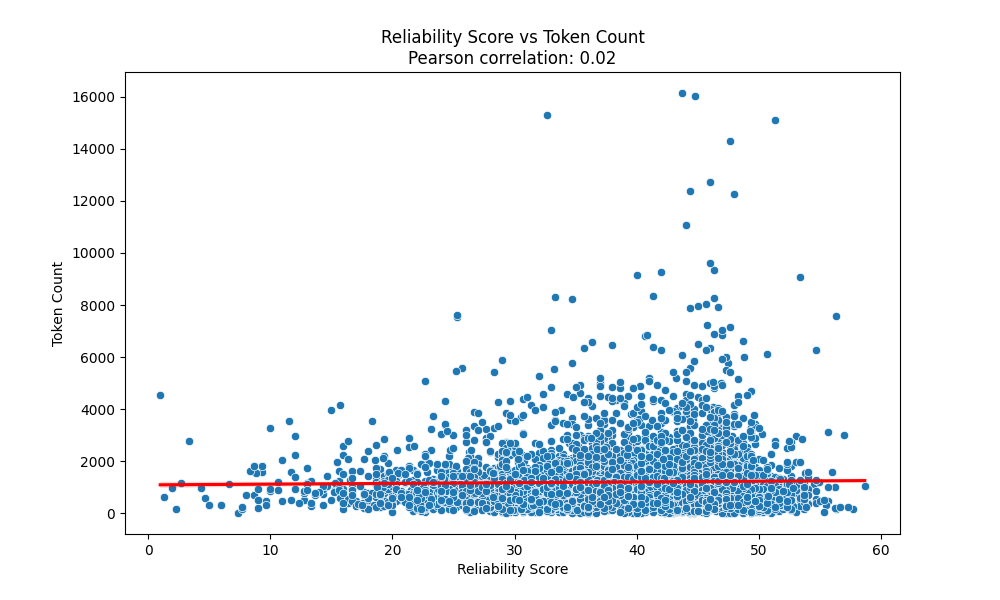
\includegraphics[width=0.7\linewidth]{figures/correlation_token_reliability_score.png}
    \caption{Pearson correlation between reliability score and token count}
    \label{fig:avg_token_pearson}
\end{figure}

Figure \ref{fig:avg_token_pearson} also shows that all classes have similar average token count, close to the overall average. The 'Problematic' and 'Questionable' classes, being the two most biased, have lower average token count than the other two classes. However, further analysis (Figure \ref{fig:avg_token_pearson}) reveals that there is virtually no linear relationship between token count and reliability score, with a Pearson correlation coefficient of 0.02. This indicates that the length of an article has no significant impact on its reliability score. In other words, longer articles are not necessarily more or less reliable than shorter ones based on the provided data.


%%% Local Variables: 
%%% mode: latex
%%% TeX-master: "thesis"
%%% End: 